Absorption spectrum of 3D and 2D materials.

\begin{parts}
	\part The series of peaks is due to excitons -- a bound state of e\textsuperscript{-}-h\textsuperscript{+} pair in a material.
	In its ground state (i.e. stationary centre-of-mass), its energy level resembles that of a hydrogen atom, hence the $-1/n^2$ dependence of $\Delta E$ in the data.
	
	\part From the graph:
	\begin{align*}
		\Delta E_1 &= 1.515-1.5188 (\unit{\electronvolt}) = -\frac{R_X}{1^2} \Rightarrow R_X = \SI{3.8}{\milli\electronvolt} \\
		\Delta E_2 &= 1.518-1.5188 (\unit{\electronvolt}) = -\frac{R_X}{2^2} \Rightarrow R_X = \SI{3.2}{\milli\electronvolt}
	\end{align*}
	Thus we have average $R_X$ of $\SI{3.5}{\milli\electronvolt}$.
	
	\part \begin{subparts}
		\subpart Larger excitonic peak in QW: due to lower dimensionality, the size of exciton decreases $\Rightarrow$ higher binding energy
		
		\subpart Step-like structure in QW: in 2D, the d.o.s. is constant $\Rightarrow$ flat structure.
		The step increase is due to the quantised harmonic level in QW, which also causes it to have a later onset than bulk.
		3D case has the usual $\sqrt{E}$ dependence in d.o.s.
	\end{subparts}
	
	\part
	\begin{figure}[H]
		\centering
		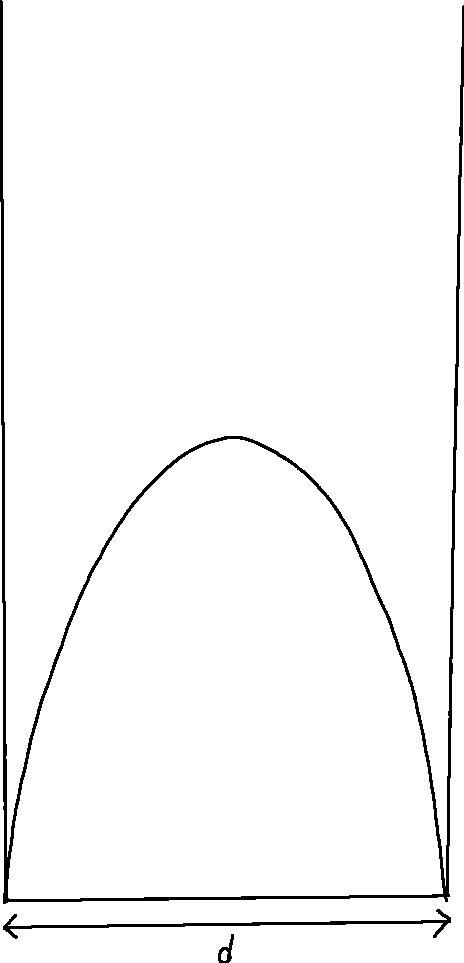
\includegraphics[width=.25\linewidth]{q2-quantum-well}
	\end{figure}
	From TISE:
	\begin{align*}
		\frac{\hat{p}^2}{2m} \psi &= E \psi \\
		\Rightarrow-\frac{\hbar^2}{2m} \frac{\mathrm{d}^2}{\mathrm{d}x^2} \psi &= E \psi \\
		\Rightarrow \textnormal{Allowed energy } E_n &= \frac{\hbar^2 k_n^2}{2m} \textnormal{\hspace{1em}where $k_n = \dfrac{n\pi}{L}$} \\
		&= \frac{\hbar^2 \pi^2 n^2}{2mL^2}
	\end{align*}
	Note that $m=m_e^*$ in conduction band, $m=m_h^*$ in valence band so we have shifted the bands by $E_n + E_n^\prime$.
	
	Selection rules for optical transitions --
	from FGL, we know the matrix element is non-zero when:
	\begin{itemize}
		\item $\psi$ and $\psi^\prime$ have the same parity $\Rightarrow$ transitions within the same oscillator level $n$.
		\item $\psi$ and $\psi^\prime$ must have sufficient overlap.
	\end{itemize}
	In addition to the dipole selection rules for bulk material.
	
	\part
	\begin{figure}[H]
		\centering
		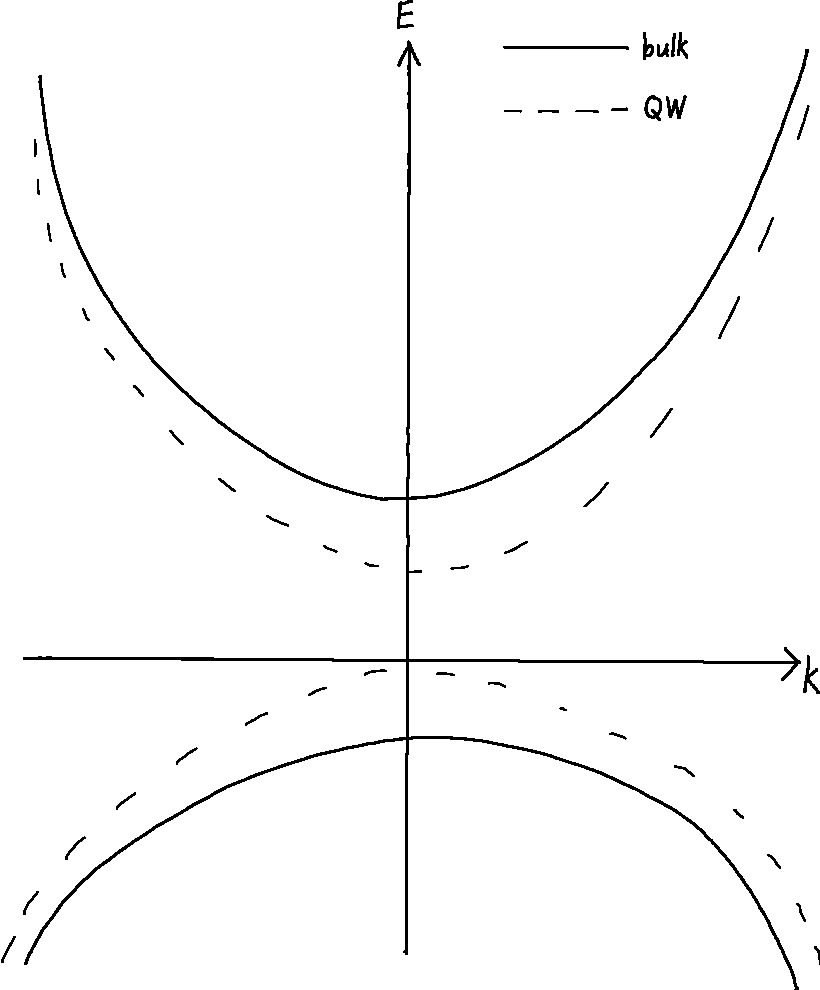
\includegraphics[width=.5\linewidth]{q2-band}
	\end{figure}
	From bulk we have $E_g \simeq \SI{1.54}{\electronvolt}$.
	
	From QW we have $E_g + E_n + E_n^\prime \simeq \SI{1.62}{\electronvolt}$ where $n=1$.
	\begin{align*}
		\Rightarrow E_1 + E_1^\prime &= \SI{0.08}{\electronvolt} \\
		&= \frac{\hbar^2 \pi^2}{2\mu L^2} \textnormal{\hspace{1em}where $\mu^{-1} = m_e^{*^{-1}} + m_{lh}^{*^{-1}}$}
	\end{align*}
	$m_{lh}^*$ is chosen since $m_{lh}^* < m_{hh}^*$ so has lower binding energy. Then:
	\begin{align*}
		\Rightarrow L^2 &= \frac{\hbar^2 \pi^2}{2\mu \left(\SI{0.08}{\electronvolt}\right)} \\
		&= \SI{7.76e-17}{\metre\squared} \\
		\Rightarrow L &= \SI{8.81}{\nano\metre}
	\end{align*}
	
	\part Optical transitions require us to have:
	\begin{align*}
		\Delta E &= E_\textnormal{conduction} - E_\textnormal{valence} \\
		&= \left(\frac{\hbar^2 k^2}{2m_e^*} + E_g\right) - \left(-\frac{\hbar^2 k^2}{2m_h^*}\right)
	\end{align*}
	where $E_g$ is a general band gap, $m_h^*$ may be either $m_{hh}^*$ or $m_{lh}^*$.
	
	\begin{align*}
		\Rightarrow \mathrm{d}E &= \frac{\hbar^2 k \, \mathrm{d}k}{\mu} \textnormal{\hspace{1em}where $\mu^{-1} = m_h^{*^{-1}} + m_e^{*^{-1}}$} \\
		k \, \mathrm{d}k &= \frac{\mu}{\hbar^2} \, \mathrm{d}E
	\end{align*}
	
	Thus in $k$ space, the joint density of transition states $N$ is:
	\begin{gather*}
		N = \int g(k) \, \mathrm{d}k \\
		\Rightarrow g(k) \, \mathrm{d}k = 2\pi k \, \mathrm{d}k \textnormal{\hspace{1em}in 2D QW} \\
		= \frac{2\pi\mu}{\hbar^2} \, \mathrm{d}E = g(E) \, \mathrm{d}E
	\end{gather*}
\end{parts}